\documentclass{article}
\usepackage[utf8]{inputenc}
\usepackage{minted}
\usepackage{graphicx}
\usepackage{lineno}
\usepackage[backend=biber,style=alphabetic,sorting=ynt]{biblatex}

\addbibresource{ref.bib}

\title{Probabilistic Machine Learning \\Sheet 1}

\author{Group 42} % Your group ID goes here
\date{03/12/2023}
\begin{document}

\maketitle
\linenumbers

\section*{Introduction Probability Theory}
All numbered sections refer to exercises listed in \cite{bishop2006pattern}, unless stated otherwise.
\subsection*{Elementary Probabilities}

\subsubsection*{2.8*}
%%% Your answers go here...
\ldots

\vspace{2em}

\subsection*{Graphical Models}

\subsubsection*{8.9*}
%%% Your answers go here...
\ldots

\subsubsection*{8.11*}
%%% Your answers go here...
\ldots


\vspace{2em}

\subsection*{Programming}
% The results of the programming Exercise should be discussed below.
% You may provide the source-code from which the results were compiled in the \textit{Code} section below.

\subsubsection*{Results}
%%% Your answers go here...
Lorem Ipsum, see Fig. \ref{fig:A}. \\
\begin{figure}[htp]
    \centering
    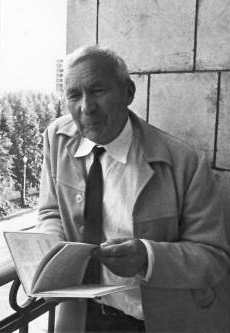
\includegraphics[width=2cm]{figures/Andrej_Nikolajewitsch_Kolmogorov.jpg}
    \caption{A.N. Kolmogorov}
    \label{fig:A}
\end{figure}


\subsubsection*{Code}
%% OPTIONAL: provide code for the programming exercise
%% Please make sure to keep the linenos option for line-numbers to reference in the review.

\begin{minted}[linenos]{python}

import numpy as np

print("Exercise PML 2023!")
# A) Create dataset by sampling 20 points and labels
x = ...
# B) Compute mean and variance of posterior
f = ...
mu = ...
var = ...
# C) Compute posterior predictive
post_predictive = ...
# D) Input points from MVN
cov_X = ...

\end{minted}
%%

\section*{Mixture Models and PPCA}

\subsection*{Theory}

\subsubsection*{9.10*}
%%% Your answers go here...
\ldots

\subsubsection*{12.4*}
%%% Your answers go here...
\ldots

\subsection*{Programming}
% The results of the programming Exercise should be discussed below.
% You may provide the source-code from which the results were compiled in the \textit{Code} section below.

\subsubsection*{Results}
%%% Your answers go here...
Lorem Ipsum \ldots \\


\printbibliography

\end{document}
